% -----------------------------------------------------
% -------- BAYSIS - Selected as Jam Initiator ---------
% -----------------------------------------------------
\subsection{BAYSIS - Selected as Jam Initiator}
\label{analysis_processing_correlation_baysis_initiator}
The correlation matrix table for the congestion-accident \textit{Jam Initiator} dataset (see \cref{table:appendix_correlation_matrix_matched_cramers}) is visual presented in \cref{img:correlation_matrix_matched_cramers} showing the the correlation of each variable combination. When visual analyzing \cref{img:correlation_matrix_matched_cramers} and checking the guidelines for a strong correlation in reference to the applied coefficient (identifiable with \cref{table:appendix_coefficient_matrix_matched}) we get a list of strongly correlated variable combinations (see \cref{tbl:correlation_list_baysis_initiator})

\noindent
\begin{table}[ht]
	\centering
	\begin{tabular}{c|l|l}  
		\toprule
		\textbf{Category} & \textbf{Strong} & \textbf{Moderate} \\
		\midrule
		Strasse & TMax, TAvg, SMax, SAvg, Cov, TLCar & \\ 
 		Kat & TMax, TAvg, SMax, SAvg & \\ 
 		Typ & SAvg, TDist, Cov & \\
 		%Betei & & \\
 		UArt1 & TMax, TAvg, SMax, SAvg, TDist, Cov, TLCar & \\
 		%UArt2 &  & \\
 		AUrs1 & TMax, TAvg, SMax, SAvg, TDist, Cov, TLHGV & \\
 		AUrs2 & TMax, TAvg, SAvg, TDist & \\
 		AufHi & TMax, TAvg, TDist, Cov & \\
 		%Alkoh & & \\
 		Char1 & TDist & \\
 		%Char2 & & \\
 		%Bes1 & & \\
 		Lich1 & TDist & \\
 		Lich2 & TDist & \\
 		Zust1 & Cov & \\
 		Zust2 & TAvg, SAvg & \\
 		%Fstf & & \\
 		%WoTag & & \\
 		%FeiTag & & \\
 		Month & SMax, Cov, TLHGV & \\
 		\bottomrule
	\end{tabular}
	\caption{List of incident variables and their strong correlated congestion variable from the congestion-accident matched data which are classified as \textit{Jam Initiator}}
	\label{tbl:correlation_list_baysis_initiator}
\end{table}

% \newgeometry{left=1.5cm,right=1cm}
% 	\pagestyle{empty}
% 	\begin{figure}[ht]
% 		\centering
% 		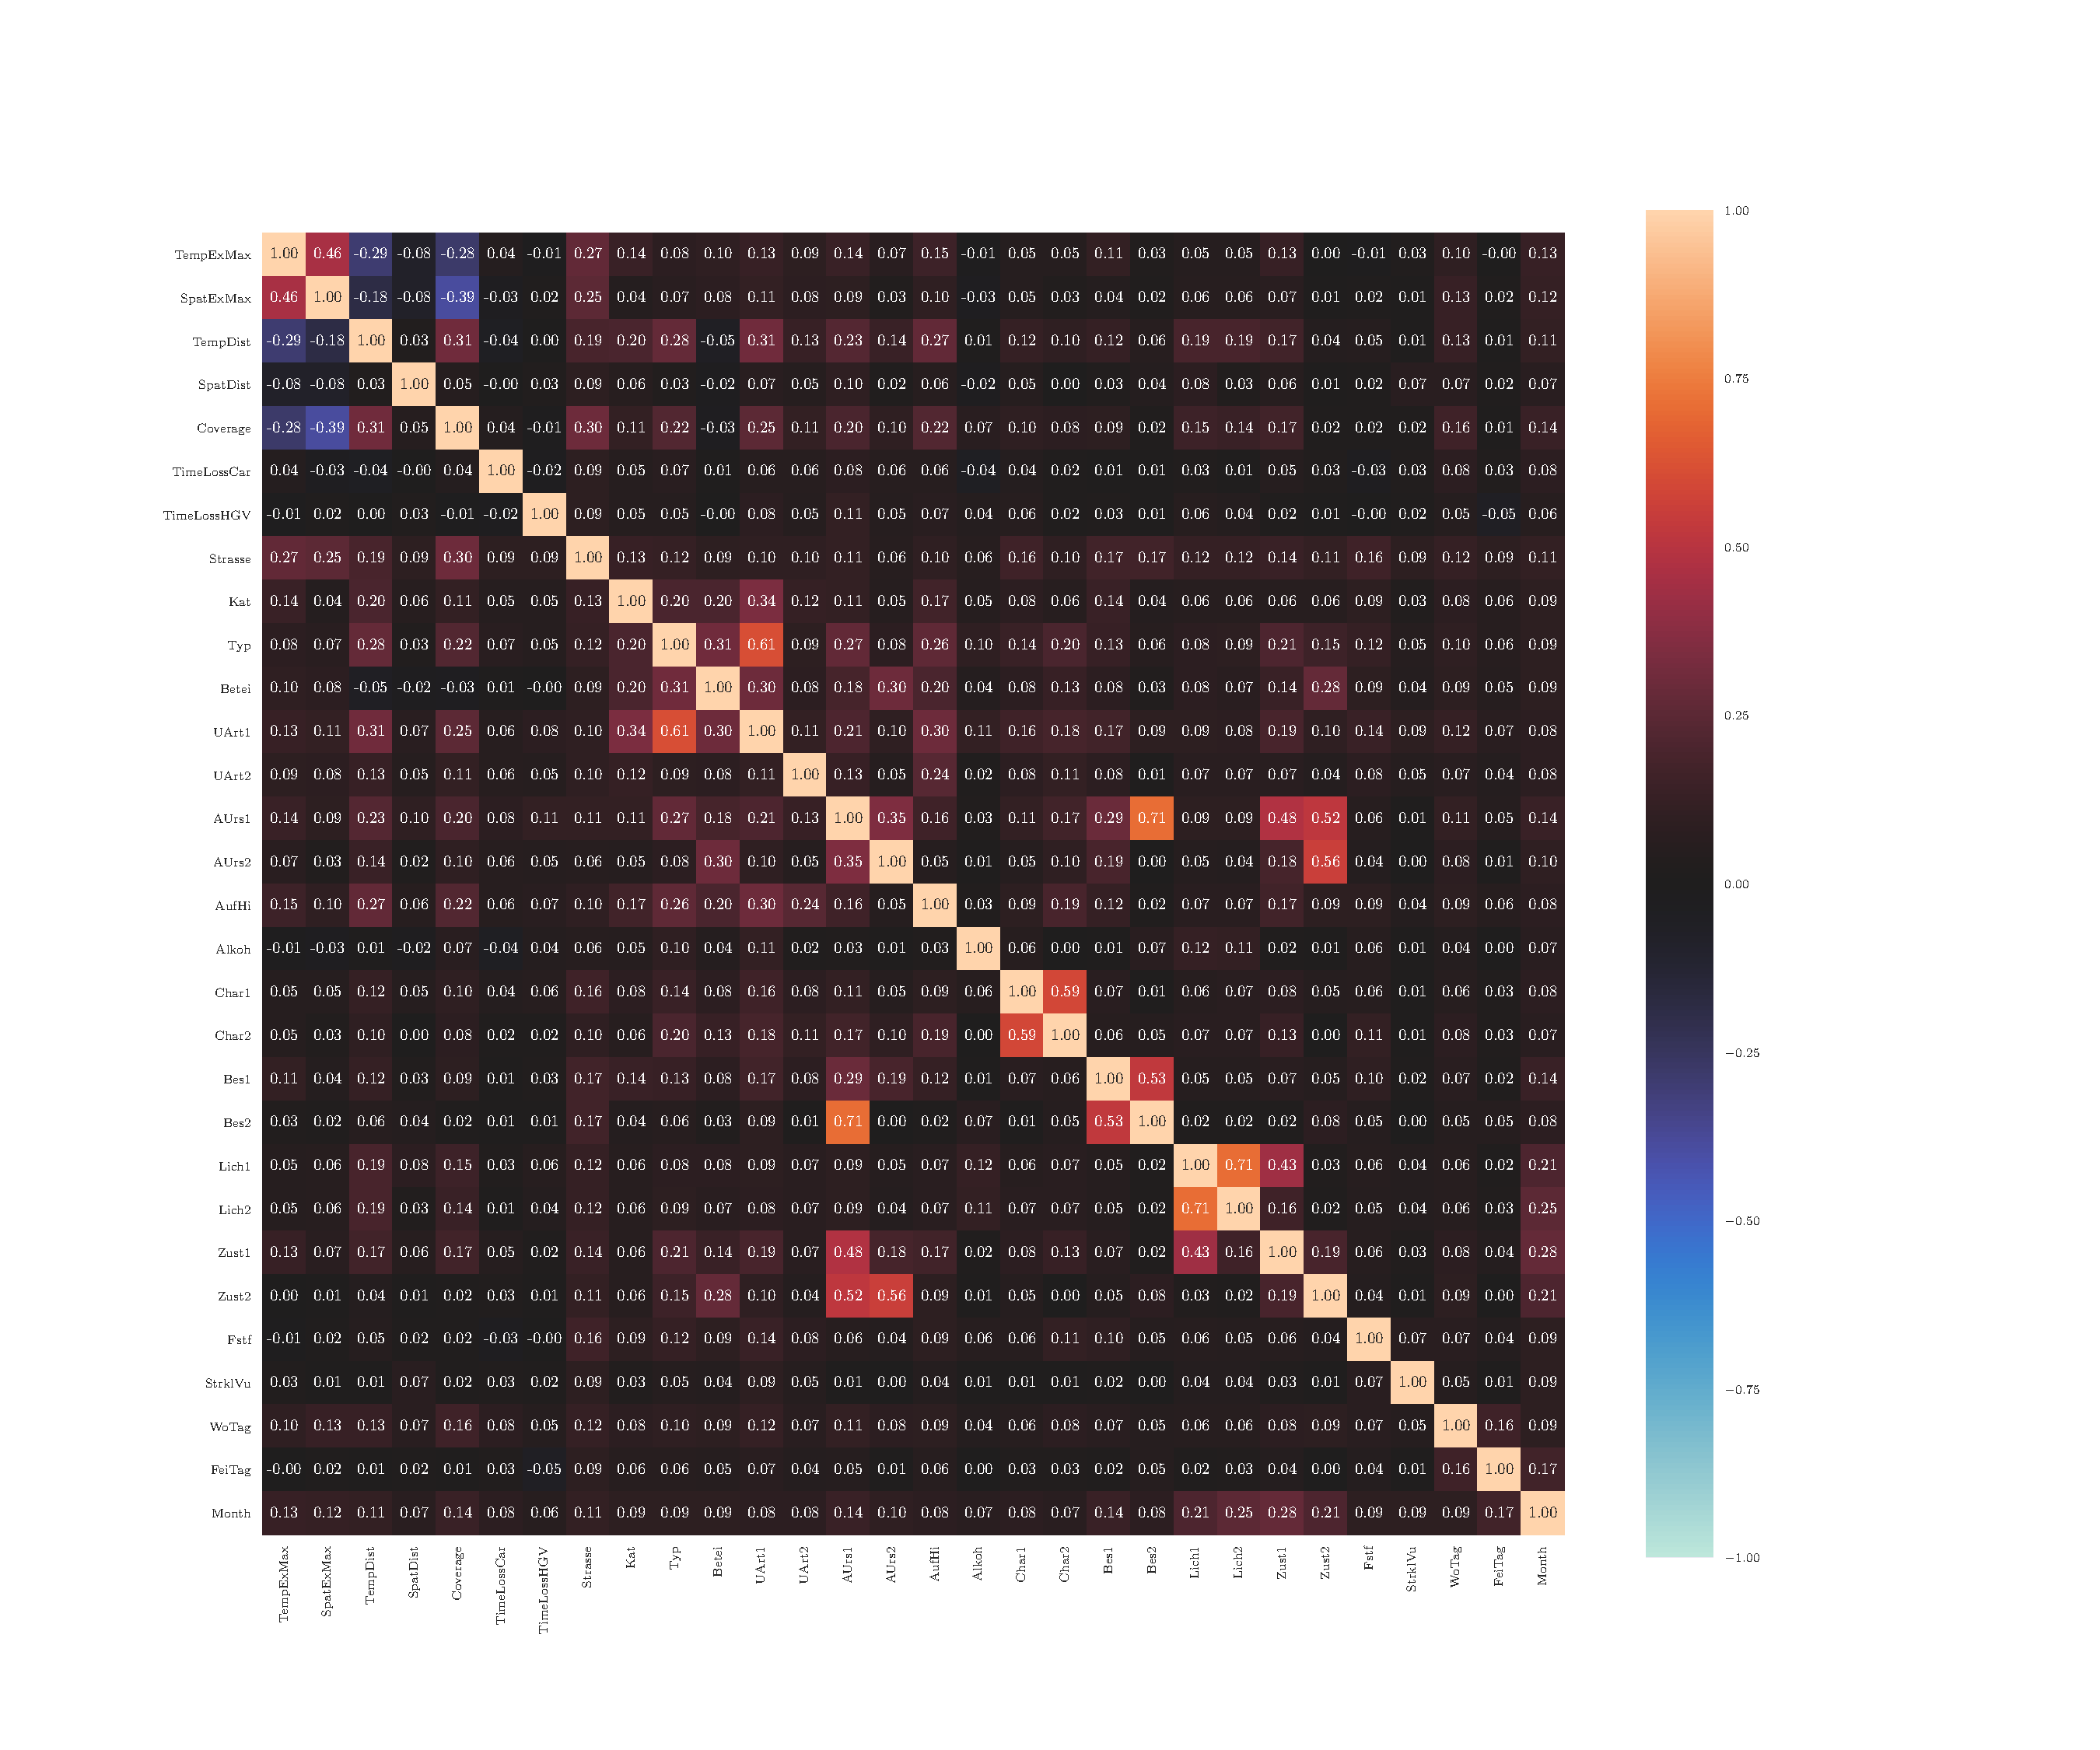
\includegraphics[scale=0.52, trim=3cm 2cm 0cm 0cm]{../CorrAnalysis/data/BAYSIS/02_matched/plots/baysis_matched_corr_cramers}
% 		\caption{Correlation matrix for BAYSIS matched data, with $V$, $\eta$, $\tau$, $r_{pq}$, $r$}
% 		\label{img:correlation_matrix_matched_cramers}
% 	\end{figure}
% \restoregeometry
\begin{figure}[!ht]
	\centering
	\makebox[\textwidth][c]{%
		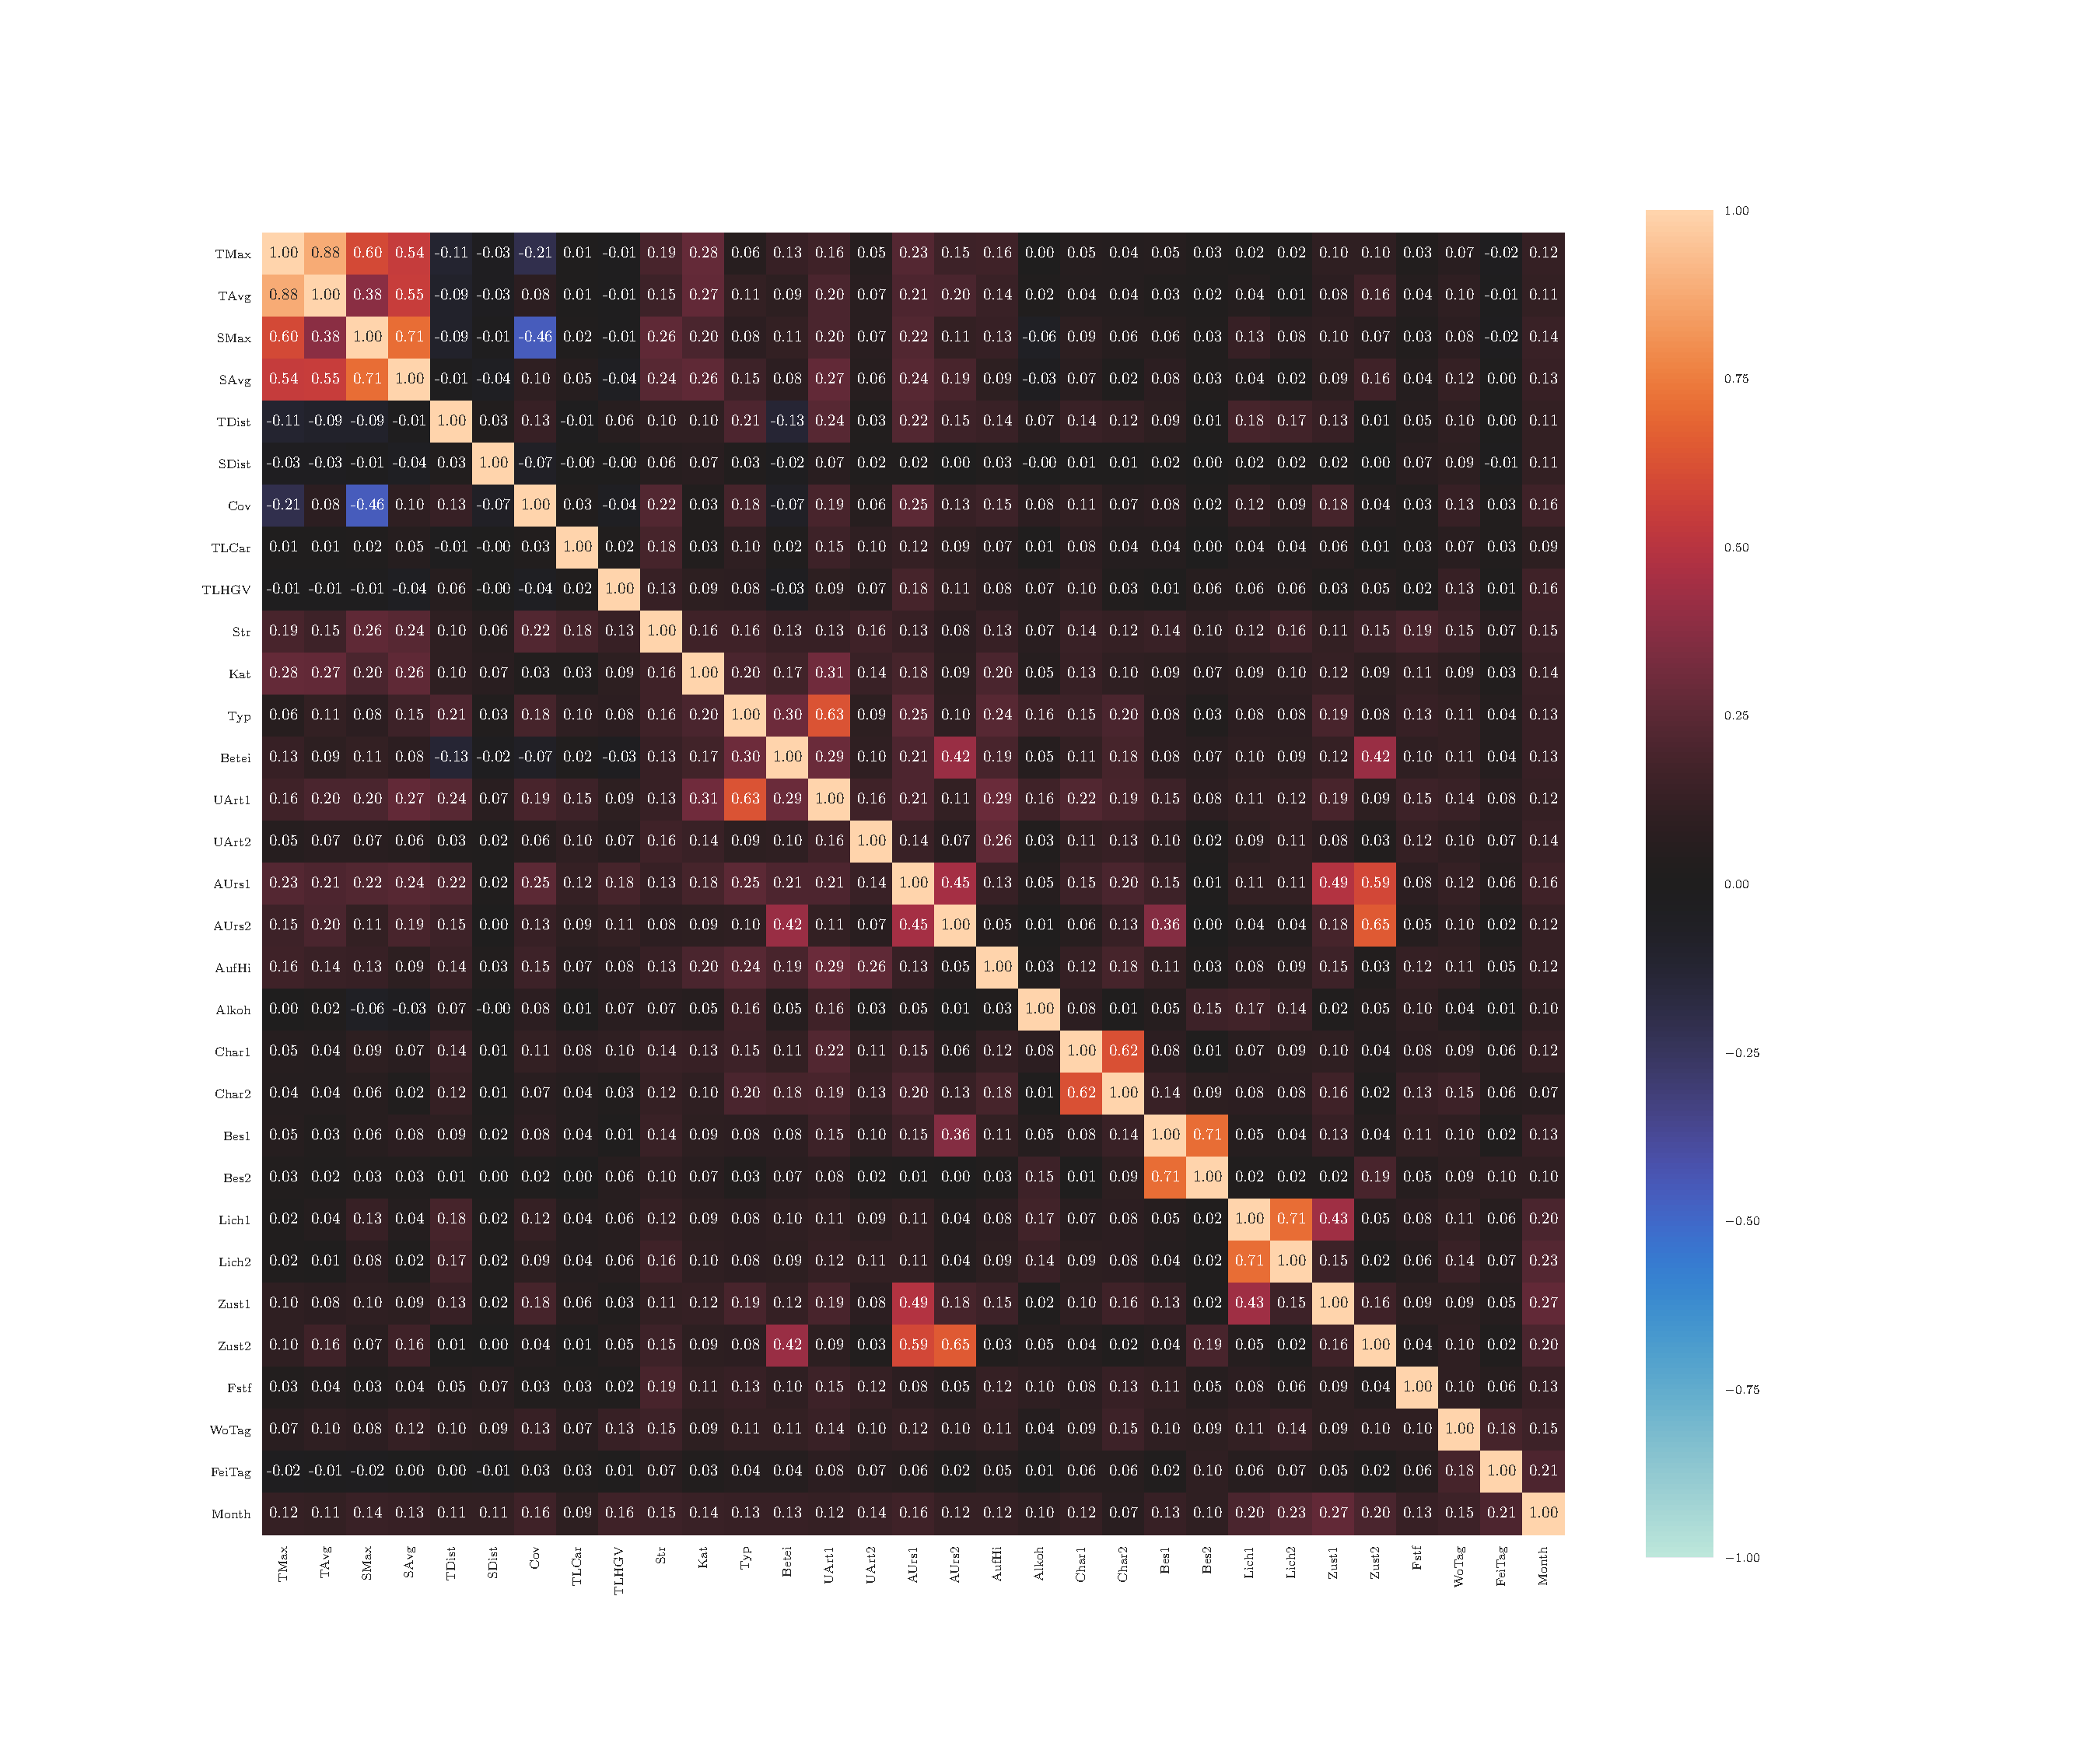
\includegraphics[width=1.4\textwidth, trim=0cm 2.5cm 6cm 3cm]{CorrAnalysis/data/BAYSIS/03_selected_01_startJam/plots/baysis_selected_corr_cramers}%
	}
	\caption{Correlation matrix for congestion-accident matched data classified as \textit{Jam Initiator}, with $V$, $\eta$, $\tau$, $r_{pq}$, $r$}
	\label{img:correlation_matrix_matched_cramers}
\end{figure}

% --------------------------
% -------- Strasse ---------
% --------------------------
\Large
\centerline{\textbf{Strasse}}
\normalsize

\paragraph{Maximal Temporal Extent}
% chi-squared = 151.97, df = 131
The Kruskal-Wallis rank sum test of \textbf{Strasse}-\textbf{TMax} produces a $p$-value of 0.1015, which is above $\alpha=.05$. The null hypothesis can't be rejected and there is \textbf{no} significant difference between the groups of \textbf{Strasse}. There are no significant groups to identify.

\paragraph{Average Temporal Extent}
% chi-squared = 173.3, df = 175
The Kruskal-Wallis rank sum test of \textbf{Strasse}-\textbf{TAvg} produces a $p$-value of 0.5221, which is above $\alpha=.05$. The null hypothesis can't be rejected and there is \textbf{no} significant difference between the groups of \textbf{Strasse}. There are no significant groups to identify.

\paragraph{Maximal Spatial Extent}
% chi-squared = 752.87, df = 720
The Kruskal-Wallis rank sum test of \textbf{Strasse}-\textbf{SMax} produces a $p$-value of 0.1919, which is above $\alpha=.05$. The null hypothesis can't be rejected and there is \textbf{no} significant difference between the groups of \textbf{Strasse}. There are no significant groups to identify.

\paragraph{Average Spatial Extent}
% chi-squared = 753.78, df = 727
The Kruskal-Wallis rank sum test of \textbf{Strasse}-\textbf{SAvg} produces a $p$-value of 0.2385, which is above $\alpha=.05$. The null hypothesis can't be rejected and there is \textbf{no} significant difference between the groups of \textbf{Strasse}. There are no significant groups to identify.

\paragraph{Coverage}
% chi-squared = 112, df = 93
The Kruskal-Wallis rank sum test of \textbf{Strasse}-\textbf{Cov} produces a $p$-value of 0.0875, which is above $\alpha=.05$. The null hypothesis can't be rejected and there is \textbf{no} significant difference between the groups of \textbf{Strasse}. There are no significant groups to identify.

\paragraph{Time-loss Car}
% chi-squared = 547.62, df = 529
The Kruskal-Wallis rank sum test of \textbf{Strasse}-\textbf{TLCar} produces a $p$-value of 0.2788, which is above $\alpha=.05$. The null hypothesis can't be rejected and there is \textbf{no} significant difference between the groups of \textbf{Strasse}. There are no significant groups to identify.


% ----------------------
% -------- Kat ---------
% ----------------------
\Large
\centerline{\textbf{Kat}}
\normalsize
This section analyzes the correlated relations of the variable \textbf{Kat} and introduces a initial interpretation of each significant correlation. Groups with an insufficient sample size (see \cref{correlation_uncertainty} are neglected and not considered. The encoding and description of the variable \textbf{Typ} is shown in \cref{tbl:baysis_dataset_Typ}.
% \begin{table}[!ht]
% 	\centering
% 	\tiny
% 	\begin{tabular}{c|l} 
% 		\toprule
% 		Code & Description \\ 
% 		\midrule
%  		0 	& Minor Accident  \\
%  		1 	& Accident with deaths  \\ 
%  		2 	& Accident with heavily injured  \\
%  		3 	& Accident with lightly injured  \\
% 		7 	& Accident with property damage  \\
% 		\bottomrule
% 	\end{tabular}
% 	\caption{Encoding of \textbf{Kat}}
% 	\label{table:analysis_encoding_Kat}
% 	%\vspace{-8mm}
% \end{table}


\paragraph{Maximal Temporal Extent}
% chi-squared = 196.02, df = 131
The Kruskal-Wallis rank sum test of \textbf{Kat}-\textbf{TMax} produces a $p$-value of 0.0002, which is way below $\alpha=.05$. The null hypothesis can therefore be rejected, which means there is a significant difference between the groups of \textbf{Kat}. To identify the significant groups, a pairwise Wilcoxon $T$-test for \textbf{Kat}-\textbf{TMax} is run, which produces \cref{tbl:wilcoxon_baysis_initiator_Kat_TMax}. 
\begin{table}[ht]
	\centering
	\begin{tabular}{c|c|c|c}
		\toprule  
  		& 1 & 2 & 3 \\ 
  		\midrule    
        2 & 0.00 &  &  \\ 
        3 & 0.00 & 0.00 &  \\ 
        7 & 0.00 & 0.00 & 0.00 \\ 
 		\bottomrule
	\end{tabular}
    \caption{Pairwise Wilcoxon $T$-test for \textit{Kat} and \textit{Maximal Temporal Extent}}
    \label{tbl:wilcoxon_baysis_initiator_Kat_TMax}
\end{table}
\todo{Explain}
\begin{table}[ht]
	\centering
	\begin{tabular}{c|c|c|c|c|c|c|c}
		\toprule  
		Group & $n$ & $\bar{x}$ & $\sigma$ & $\tilde{x}$ & $min$ & $max$ & $\Delta$ \\
        \midrule
        1 & 29  & 290.07 & 190.59 & 255.00 & 27 & 864  & 837 \\ 
        2 & 144 & 156.23 & 119.44 & 120.00 & 9  & 657  & 648 \\ 
        3 & 423 & 121.05 & 105.34 & 99.00  & 9  & 1116 & 1107 \\ 
        7 & 181 & 103.13 & 143.89 & 75.00  & 9  & 1341 & 1332 \\ 
 		\bottomrule
	\end{tabular}
    \caption{Descriptives of the groups of \textit{Kat} and \textit{Maximal Temporal Extent}}
    \label{tbl:descriptives_baysis_initiator_Kat_TMax}
\end{table}

\paragraph{Average temporal Extent}
% chi-squared = 222.52, df = 175
The Kruskal-Wallis rank sum test of \textbf{Kat}-\textbf{TAvg} produces a $p$-value of 0.0087, which is way below $\alpha=.05$. The null hypothesis can therefore be rejected, which means there is a significant difference between the groups of \textbf{Kat}. To identify the significant groups, a pairwise Wilcoxon $T$-test for \textbf{Kat}-\textbf{TAvg} is run, which produces \cref{tbl:wilcoxon_baysis_initiator_Kat_TAvg}. 
\begin{table}[ht]
	\small
	\centering
    \begin{tabular}{rrrr}
        \toprule
        & 1 & 2 & 3 \\ 
        \midrule
        2 & 0.00 &  &  \\ 
        3 & 0.00 & 0.01 &  \\ 
        7 & 0.00 & 0.00 & 0.00 \\ 
        \bottomrule
    \end{tabular}
	\caption{Pairwise Wilcoxon $T$-test for \textit{Kat} and \textit{Average Temporal Extent}}
	\label{tbl:wilcoxon_baysis_initiator_Kat_TAvg}
\end{table}
\todo{Explain}
\begin{table}[ht]
	\small
	\centering
    \begin{tabular}{rrrrrrrrrrrrrr}
        \toprule
        Group & $n$ & $\bar{x}$ & $\sigma$ & $\tilde{x}$ & $min$ & $max$ & $\Delta$ \\
        \midrule
        1 & 29  & 148.76 & 90.65 & 144.00 & 20 & 376 & 356 \\ 
        2 & 144 & 80.91  & 67.52 & 61.50  & 7  & 426 & 419 \\ 
        3 & 423 & 63.84  & 51.24 & 53.00  & 5  & 469 & 464 \\ 
        7 & 181 & 53.61  & 80.96 & 39.00  & 4  & 920 & 916 \\ 
        \bottomrule
    \end{tabular}
	\caption{Group descriptives of \textit{Kat} and \textit{Average temporal Extent}}
	\label{tbl:descriptives_baysis_initiator_Kat_TAvg}
	%\vspace{-8mm}
\end{table}

\paragraph{Maximal spatial Extent}
% chi-squared = 732.27, df = 720
The Kruskal-Wallis rank sum test of \textbf{Kat}-\textbf{SMax} produces a $p$-value of 0.3673, which is above $\alpha=.05$. The null hypothesis can't be rejected and there is \textbf{no} significant difference between the groups of \textbf{Kat}. There are no significant groups to identify.

\paragraph{Average spatial Extent}
% chi-squared = 738.37, df = 727
The Kruskal-Wallis rank sum test of \textbf{Kat}-\textbf{SAvg} produces a $p$-value of 0.3767, which is above $\alpha=.05$. The null hypothesis can't be rejected and there is \textbf{no} significant difference between the groups of \textbf{Kat}. There are no significant groups to identify.

% ----------------------
% -------- Typ ---------
% ----------------------
\Large
\centerline{\textbf{Typ}}
\normalsize

\paragraph{Average spatial Extent}
% chi-squared = 739.95, df = 727
The Kruskal-Wallis rank sum test of \textbf{Kat}-\textbf{SAvg} produces a $p$-value of 0.3613, which is above $\alpha=.05$. The null hypothesis can't be rejected and there is \textbf{no} significant difference between the groups of \textbf{Kat}. There are no significant groups to identify.

\paragraph{Temporal Distance}
% chi-squared = 39.181, df = 24
The Kruskal-Wallis rank sum test of \textbf{Kat}-\textbf{TDist} produces a $p$-value of 0.0261, which is way below $\alpha=.05$. The null hypothesis can therefore be rejected, which means there is a significant difference between the groups of \textbf{Kat}. To identify the significant groups, a pairwise Wilcoxon $T$-test for \textbf{Kat}-\textbf{TDist} is run, which produces \cref{tbl:wilcoxon_baysis_initiator_Typ_TDist}. 
\begin{table}[ht]
	\small
	\centering
    \begin{tabular}{rrrrrr}
        \toprule
        & 1 & 3 & 4 & 5 & 6 \\ 
        \midrule
        3 & 0.05 &  &  &  &  \\ 
        4 & 1.00 & 0.38 &  &  &  \\ 
        5 & 0.96 & 1.00 & 0.96 &  &  \\ 
        6 & 0.00 & 0.96 & 0.51 & 1.00 &  \\ 
        7 & 1.00 & 0.04 & 1.00 & 0.96 & 0.01 \\ 
        \bottomrule
    \end{tabular}
    \caption{Pairwise Wilcoxon $T$-test for \textit{Typ} and \textit{Temporal Distance}}
    \label{tbl:wilcoxon_baysis_initiator_Typ_TDist}
\end{table}
\todo{Explain}
\begin{table}[ht]
	\small
	\centering
    \begin{tabular}{rrrrrrrrrrrrrr}
        \toprule
        Group & $n$ & $\bar{x}$ & $\sigma$ & $\tilde{x}$ & $min$ & $max$ & $\Delta$ \\
        \midrule
        1 & 181 & 11.40 & 6.38 & 10.00 & 1  & 24 & 23 \\ 
        3 & 24  & 7.67  & 6.06 & 7.00  & 1  & 22 & 21 \\ 
        4 & 4   & 14.00 & 3.92 & 13.50 & 10 & 19 & 9 \\ 
        5 & 2   & 4.50  & 3.54 & 4.50  & 2  & 7  & 5 \\ 
        6 & 496 & 9.20  & 5.88 & 8.00  & 0  & 24 & 24 \\ 
        7 & 70  & 12.27 & 7.09 & 11.00 & 0  & 24 & 24 \\ 
        \bottomrule
    \end{tabular}
    \caption{Group descriptives of \textit{Typ} and \textit{Temporal Distance}}
    \label{tbl:descriptives_baysis_initiator_Typ_TDist}
	%\vspace{-8mm}
\end{table}

\paragraph{Coverage}
% chi-squared = 87.648, df = 93
The Kruskal-Wallis rank sum test of \textbf{Kat}-\textbf{Cov} produces a $p$-value of 0.6372, which is above $\alpha=.05$. The null hypothesis can't be rejected and there is \textbf{no} significant difference between the groups of \textbf{Kat}. There are no significant groups to identify.

% ------------------------
% -------- UArt1 ---------
% ------------------------
\Large
\centerline{\textbf{UArt1}}
\normalsize

\paragraph{Maximal Temporal Extent}
Kruskal-Wallis chi-squared = 184.29, df = 131, p-value = 0.001496

% latex table generated in R 4.0.2 by xtable 1.8-4 package
% 
\begin{tabular}{rrrrrrrrrr}
  \hline
 & 0 & 1 & 2 & 3 & 4 & 5 & 6 & 7 & 8 \\ 
  \hline
1 & 1.00 &  &  &  &  &  &  &  &  \\ 
  2 & 1.00 & 1.00 &  &  &  &  &  &  &  \\ 
  3 & 1.00 & 0.04 & 0.00 &  &  &  &  &  &  \\ 
  4 & 1.00 & 1.00 & 1.00 & 1.00 &  &  &  &  &  \\ 
  5 & 1.00 & 1.00 & 1.00 & 1.00 & 1.00 &  &  &  &  \\ 
  6 & 1.00 & 1.00 & 1.00 & 1.00 & 1.00 & 1.00 &  &  &  \\ 
  7 & 0.75 & 0.05 & 0.12 & 1.00 & 1.00 & 1.00 & 1.00 &  &  \\ 
  8 & 1.00 & 0.21 & 0.43 & 1.00 & 1.00 & 1.00 & 1.00 & 1.00 &  \\ 
  9 & 1.00 & 0.43 & 1.00 & 1.00 & 1.00 & 1.00 & 1.00 & 1.00 & 1.00 \\ 
   \hline
\end{tabular}
% latex table generated in R 4.0.2 by xtable 1.8-4 package
% 
\begin{tabular}{rrrrrrrrrrrrrr}
  \hline
 & vars & n & mean & sd & median & trimmed & mad & min & max & range & skew & kurtosis & se \\ 
  \hline
X1 & 1.00 & 24.00 & 140.75 & 100.75 & 114.00 & 129.00 & 57.82 & 30.00 & 375.00 & 345.00 & 1.16 & 0.00 & 20.57 \\ 
  X11 & 1.00 & 31.00 & 198.58 & 166.25 & 126.00 & 173.64 & 111.19 & 39.00 & 612.00 & 573.00 & 1.12 & 0.03 & 29.86 \\ 
  X12 & 1.00 & 345.00 & 134.87 & 108.69 & 105.00 & 116.33 & 57.82 & 9.00 & 864.00 & 855.00 & 2.49 & 9.12 & 5.85 \\ 
  X13 & 1.00 & 144.00 & 111.79 & 123.13 & 81.00 & 89.97 & 53.37 & 9.00 & 1116.00 & 1107.00 & 4.48 & 29.82 & 10.26 \\ 
  X14 & 1.00 & 4.00 & 186.00 & 145.68 & 175.50 & 186.00 & 162.34 & 39.00 & 354.00 & 315.00 & 0.09 & -2.24 & 72.84 \\ 
  X15 & 1.00 & 15.00 & 179.60 & 324.31 & 99.00 & 102.92 & 17.79 & 15.00 & 1341.00 & 1326.00 & 3.03 & 7.98 & 83.74 \\ 
  X16 & 1.00 & 4.00 & 171.00 & 98.62 & 178.50 & 171.00 & 113.42 & 66.00 & 261.00 & 195.00 & -0.05 & -2.37 & 49.31 \\ 
  X17 & 1.00 & 23.00 & 87.91 & 93.15 & 48.00 & 71.53 & 44.48 & 12.00 & 384.00 & 372.00 & 1.57 & 2.07 & 19.42 \\ 
  X18 & 1.00 & 107.00 & 118.46 & 117.62 & 87.00 & 97.00 & 57.82 & 18.00 & 813.00 & 795.00 & 3.25 & 13.70 & 11.37 \\ 
  X19 & 1.00 & 80.00 & 122.47 & 143.91 & 91.50 & 98.58 & 55.60 & 12.00 & 1152.00 & 1140.00 & 5.14 & 31.86 & 16.09 \\ 
   \hline
\end{tabular}
\paragraph{Average Temporal Extent}
Kruskal-Wallis chi-squared = 182.51, df = 175, p-value = 0.3331
\paragraph{Maximal Spatial Extent}
Kruskal-Wallis chi-squared = 735.57, df = 720, p-value = 0.3355
\paragraph{Average Spatial Extent}
Kruskal-Wallis chi-squared = 741.73, df = 727, p-value = 0.3442
\paragraph{Temporal Distance}
Kruskal-Wallis chi-squared = 43.627, df = 24, p-value = 0.008429

% latex table generated in R 4.0.2 by xtable 1.8-4 package
% 
\begin{tabular}{rrrrrrrrrr}
  \hline
 & 0 & 1 & 2 & 3 & 4 & 5 & 6 & 7 & 8 \\ 
  \hline
1 & 1.00 &  &  &  &  &  &  &  &  \\ 
  2 & 1.00 & 1.00 &  &  &  &  &  &  &  \\ 
  3 & 1.00 & 1.00 & 1.00 &  &  &  &  &  &  \\ 
  4 & 1.00 & 1.00 & 1.00 & 1.00 &  &  &  &  &  \\ 
  5 & 1.00 & 1.00 & 1.00 & 1.00 & 1.00 &  &  &  &  \\ 
  6 & 1.00 & 1.00 & 1.00 & 1.00 & 1.00 & 1.00 &  &  &  \\ 
  7 & 1.00 & 0.06 & 0.00 & 0.00 & 1.00 & 0.10 & 1.00 &  &  \\ 
  8 & 1.00 & 1.00 & 0.01 & 0.01 & 1.00 & 1.00 & 1.00 & 1.00 &  \\ 
  9 & 1.00 & 1.00 & 0.05 & 0.01 & 1.00 & 0.78 & 1.00 & 0.87 & 1.00 \\ 
   \hline
\end{tabular}
% latex table generated in R 4.0.2 by xtable 1.8-4 package
% 
\begin{tabular}{rrrrrrrrrrrrrr}
  \hline
 & vars & n & mean & sd & median & trimmed & mad & min & max & range & skew & kurtosis & se \\ 
  \hline
X1 & 1.00 & 24.00 & 11.04 & 6.22 & 10.00 & 10.85 & 8.15 & 2.00 & 22.00 & 20.00 & 0.25 & -1.33 & 1.27 \\ 
  X11 & 1.00 & 31.00 & 8.94 & 6.03 & 7.00 & 8.28 & 5.93 & 0.00 & 24.00 & 24.00 & 0.88 & 0.08 & 1.08 \\ 
  X12 & 1.00 & 345.00 & 9.21 & 5.90 & 8.00 & 8.62 & 4.45 & 1.00 & 24.00 & 23.00 & 0.80 & -0.16 & 0.32 \\ 
  X13 & 1.00 & 144.00 & 8.80 & 6.03 & 7.00 & 7.99 & 4.45 & 1.00 & 24.00 & 23.00 & 1.15 & 0.48 & 0.50 \\ 
  X14 & 1.00 & 4.00 & 12.00 & 4.08 & 10.50 & 12.00 & 1.48 & 9.00 & 18.00 & 9.00 & 0.66 & -1.75 & 2.04 \\ 
  X15 & 1.00 & 15.00 & 8.13 & 7.06 & 7.00 & 7.69 & 4.45 & 0.00 & 22.00 & 22.00 & 0.86 & -0.67 & 1.82 \\ 
  X16 & 1.00 & 4.00 & 14.00 & 3.92 & 13.50 & 14.00 & 3.71 & 10.00 & 19.00 & 9.00 & 0.22 & -2.05 & 1.96 \\ 
  X17 & 1.00 & 23.00 & 15.26 & 7.04 & 14.00 & 15.47 & 10.38 & 4.00 & 24.00 & 20.00 & -0.11 & -1.67 & 1.47 \\ 
  X18 & 1.00 & 107.00 & 11.81 & 6.57 & 11.00 & 11.62 & 7.41 & 1.00 & 24.00 & 23.00 & 0.26 & -1.07 & 0.63 \\ 
  X19 & 1.00 & 80.00 & 11.38 & 5.87 & 10.00 & 10.98 & 5.93 & 2.00 & 24.00 & 22.00 & 0.53 & -0.69 & 0.66 \\ 
   \hline
\end{tabular}
\paragraph{Coverage}
Kruskal-Wallis chi-squared = 119.45, df = 93, p-value = 0.0337

% latex table generated in R 4.0.2 by xtable 1.8-4 package
% 
\begin{tabular}{rrrrrrrrrr}
  \hline
 & 0 & 1 & 2 & 3 & 4 & 5 & 6 & 7 & 8 \\ 
  \hline
1 & 1.00 &  &  &  &  &  &  &  &  \\ 
  2 & 1.00 & 1.00 &  &  &  &  &  &  &  \\ 
  3 & 1.00 & 1.00 & 1.00 &  &  &  &  &  &  \\ 
  4 & 1.00 & 1.00 & 1.00 & 1.00 &  &  &  &  &  \\ 
  5 & 1.00 & 1.00 & 1.00 & 1.00 & 1.00 &  &  &  &  \\ 
  6 & 1.00 & 1.00 & 1.00 & 1.00 & 1.00 & 1.00 &  &  &  \\ 
  7 & 1.00 & 1.00 & 1.00 & 1.00 & 1.00 & 1.00 & 1.00 &  &  \\ 
  8 & 1.00 & 1.00 & 0.12 & 0.09 & 1.00 & 0.72 & 1.00 & 1.00 &  \\ 
  9 & 1.00 & 1.00 & 1.00 & 1.00 & 1.00 & 1.00 & 1.00 & 1.00 & 1.00 \\ 
   \hline
\end{tabular}
% latex table generated in R 4.0.2 by xtable 1.8-4 package
% 
\begin{tabular}{rrrrrrrrrrrrrr}
  \hline
 & vars & n & mean & sd & median & trimmed & mad & min & max & range & skew & kurtosis & se \\ 
  \hline
X1 & 1.00 & 24.00 & 51.38 & 20.70 & 45.50 & 50.15 & 20.76 & 23.00 & 96.00 & 73.00 & 0.49 & -1.07 & 4.23 \\ 
  X11 & 1.00 & 31.00 & 53.68 & 18.85 & 50.00 & 51.96 & 14.83 & 28.00 & 96.00 & 68.00 & 0.75 & -0.43 & 3.38 \\ 
  X12 & 1.00 & 345.00 & 50.71 & 19.95 & 50.00 & 50.15 & 22.24 & 7.00 & 100.00 & 93.00 & 0.22 & -0.58 & 1.07 \\ 
  X13 & 1.00 & 144.00 & 48.90 & 19.87 & 50.00 & 48.85 & 19.27 & 5.00 & 98.00 & 93.00 & 0.02 & -0.27 & 1.66 \\ 
  X14 & 1.00 & 4.00 & 58.00 & 21.10 & 59.00 & 58.00 & 25.20 & 36.00 & 78.00 & 42.00 & -0.03 & -2.37 & 10.55 \\ 
  X15 & 1.00 & 15.00 & 43.27 & 21.32 & 42.00 & 42.23 & 23.72 & 12.00 & 88.00 & 76.00 & 0.43 & -0.77 & 5.51 \\ 
  X16 & 1.00 & 4.00 & 74.75 & 18.93 & 80.50 & 74.75 & 11.12 & 48.00 & 90.00 & 42.00 & -0.52 & -1.87 & 9.46 \\ 
  X17 & 1.00 & 23.00 & 59.09 & 25.74 & 62.00 & 59.16 & 32.62 & 18.00 & 100.00 & 82.00 & -0.03 & -1.39 & 5.37 \\ 
  X18 & 1.00 & 107.00 & 58.85 & 23.92 & 57.00 & 58.74 & 25.20 & 7.00 & 100.00 & 93.00 & 0.06 & -0.91 & 2.31 \\ 
  X19 & 1.00 & 80.00 & 56.73 & 21.86 & 54.00 & 56.03 & 25.20 & 18.00 & 100.00 & 82.00 & 0.25 & -1.10 & 2.44 \\ 
   \hline
\end{tabular}
\paragraph{Time-Loss Car}
Kruskal-Wallis chi-squared = 525, df = 529, p-value = 0.5409

% ------------------------
% -------- AUrs1 ---------
% ------------------------
\Large
\centerline{\textbf{AUrs1}}
\normalsize

\paragraph{Maximal Temporal Extent}
% chi-squared = 136.52, df = 131
The Kruskal-Wallis rank sum test of \textbf{AUrs1}-\textbf{TMax} produces a $p$-value of 0.3529, which is above $\alpha=.05$. The null hypothesis can't be rejected and there is \textbf{no} significant difference between the groups of \textbf{AUrs1}. There are no significant groups to identify.
\paragraph{Average Temporal Extent}
% chi-squared = 205.3, df = 175
The Kruskal-Wallis rank sum test of \textbf{AUrs1}-\textbf{TMax} produces a $p$-value of 0.05823, which is above $\alpha=.05$. The null hypothesis can't be rejected and there is \textbf{no} significant difference between the groups of \textbf{AUrs1}. There are no significant groups to identify.
\paragraph{Maximal Spatial Extent}
% chi-squared = 746.53, df = 720
The Kruskal-Wallis rank sum test of \textbf{AUrs1}-\textbf{TMax} produces a $p$-value of 0.2394, which is above $\alpha=.05$. The null hypothesis can't be rejected and there is \textbf{no} significant difference between the groups of \textbf{AUrs1}. There are no significant groups to identify.
\paragraph{Average Spatial Extent}
% chi-squared = 734.88, df = 727
The Kruskal-Wallis rank sum test of \textbf{AUrs1}-\textbf{TMax} produces a $p$-value of 0.4117, which is above $\alpha=.05$. The null hypothesis can't be rejected and there is \textbf{no} significant difference between the groups of \textbf{AUrs1}. There are no significant groups to identify.
\paragraph{Temporal Distance}
% chi-squared = 31.402, df = 24
The Kruskal-Wallis rank sum test of \textbf{AUrs1}-\textbf{TMax} produces a $p$-value of 0.1425, which is above $\alpha=.05$. The null hypothesis can't be rejected and there is \textbf{no} significant difference between the groups of \textbf{AUrs1}. There are no significant groups to identify.
\paragraph{Coverage}
% chi-squared = 123.97, df = 93, p-value = 0.0176

\begin{table}[ht]
	\small
	\centering
    \begin{tabular}{rrrrrrrrrrrrr}
        \hline
        & 0 & 72 & 73 & 75 & 77 & 81 & 82 & 83 & 84 & 86 & 87 & 88 \\ 
        \hline
        72 & 0.01 &  &  &  &  &  &  &  &  &  &  &  \\ 
        73 & 0.24 & 0.63 &  &  &  &  &  &  &  &  &  &  \\ 
        75 & 1.00 & 1.00 & 1.00 &  &  &  &  &  &  &  &  &  \\ 
        77 & 1.00 & 1.00 & 1.00 & 1.00 &  &  &  &  &  &  &  &  \\ 
        81 & 1.00 & 1.00 & 1.00 & 1.00 & 1.00 &  &  &  &  &  &  &  \\ 
        82 & 1.00 & 1.00 & 1.00 & 1.00 & 1.00 & 1.00 &  &  &  &  &  &  \\ 
        83 & 1.00 & 1.00 & 1.00 & 1.00 & 1.00 & 1.00 & 1.00 &  &  &  &  &  \\ 
        84 & 1.00 & 1.00 & 1.00 & 1.00 & 1.00 & 1.00 & 1.00 & 1.00 &  &  &  &  \\ 
        86 & 1.00 & 1.00 & 1.00 & 1.00 & 1.00 & 1.00 & 1.00 & 1.00 & 1.00 &  &  &  \\ 
        87 & 1.00 & 1.00 & 1.00 & 1.00 & 1.00 & 1.00 & 1.00 & 1.00 & 1.00 & 1.00 &  &  \\ 
        88 & 1.00 & 1.00 & 1.00 & 1.00 & 1.00 & 1.00 & 1.00 & 1.00 & 1.00 & 1.00 & 1.00 &  \\ 
        89 & 1.00 & 0.33 & 0.96 & 1.00 & 1.00 & 1.00 & 1.00 & 1.00 & 1.00 & 0.91 & 1.00 & 1.00 \\ 
        \hline
    \end{tabular}
    \caption{Pairwise Wilcoxon $T$-test for \textit{AUrs1} and \textit{Coverage}}
    \label{tbl:wilcoxon_baysis_initiator_AUrs1_Cov}
\end{table}
\todo{Explain}
\begin{table}[ht]
	\small
	\centering
    \begin{tabular}{rrrrrrrrrrrrrr}
        \hline
        & vars & n & mean & sd & median & trimmed & mad & min & max & range & skew & kurtosis & se \\ 
        \hline
        X1 & 1.00 & 663.00 & 51.10 & 20.67 & 50.00 & 50.39 & 20.76 & 5.00 & 100.00 & 95.00 & 0.26 & -0.46 & 0.80 \\ 
        X11 & 1.00 & 20.00 & 72.75 & 26.16 & 87.50 & 76.00 & 9.64 & 20.00 & 100.00 & 80.00 & -0.94 & -0.69 & 5.85 \\ 
        X12 & 1.00 & 63.00 & 59.16 & 20.47 & 59.00 & 59.43 & 23.72 & 15.00 & 100.00 & 85.00 & -0.08 & -0.81 & 2.58 \\ 
        X13 & 1.00 & 1.00 & 100.00 &  & 100.00 & 100.00 & 0.00 & 100.00 & 100.00 & 0.00 &  &  &  \\ 
        X14 & 1.00 & 1.00 & 79.00 &  & 79.00 & 79.00 & 0.00 & 79.00 & 79.00 & 0.00 &  &  &  \\ 
        X15 & 1.00 & 3.00 & 61.67 & 26.10 & 59.00 & 61.67 & 32.62 & 37.00 & 89.00 & 52.00 & 0.10 & -2.33 & 15.07 \\ 
        X16 & 1.00 & 5.00 & 43.20 & 7.22 & 45.00 & 43.20 & 8.90 & 33.00 & 51.00 & 18.00 & -0.29 & -1.87 & 3.23 \\ 
        X17 & 1.00 & 1.00 & 76.00 &  & 76.00 & 76.00 & 0.00 & 76.00 & 76.00 & 0.00 &  &  &  \\ 
        X18 & 1.00 & 1.00 & 32.00 &  & 32.00 & 32.00 & 0.00 & 32.00 & 32.00 & 0.00 &  &  &  \\ 
        X19 & 1.00 & 3.00 & 83.00 & 13.00 & 90.00 & 83.00 & 1.48 & 68.00 & 91.00 & 23.00 & -0.38 & -2.33 & 7.51 \\ 
        X110 & 1.00 & 1.00 & 67.00 &  & 67.00 & 67.00 & 0.00 & 67.00 & 67.00 & 0.00 &  &  &  \\ 
        X111 & 1.00 & 4.00 & 66.50 & 26.56 & 71.00 & 66.50 & 25.95 & 35.00 & 89.00 & 54.00 & -0.16 & -2.26 & 13.28 \\ 
        X112 & 1.00 & 11.00 & 43.45 & 11.22 & 42.00 & 43.44 & 8.90 & 25.00 & 62.00 & 37.00 & 0.21 & -0.95 & 3.38 \\ 
        \hline
      \end{tabular}
    \caption{Group descriptives of \textit{AUrs1} and \textit{Coverage}}
    \label{tbl:descriptives_baysis_initiator_AUrs1_Cov}
	%\vspace{-8mm}
\end{table}

\paragraph{Time-loss HGV}
% chi-squared = 416.29, df = 391
The Kruskal-Wallis rank sum test of \textbf{AUrs1}-\textbf{TLHGV} produces a $p$-value of 0.1816, which is above $\alpha=.05$. The null hypothesis can't be rejected and there is \textbf{no} significant difference between the groups of \textbf{AUrs1}. There are no significant groups to identify.

\medskip
Next the second \textbf{AUrs} variable will be tested.
\medskip

\paragraph{Maximal Temporal Extent}
% chi-squared = 105.63, df = 131
The Kruskal-Wallis rank sum test of \textbf{AUrs2}-\textbf{TMax} produces a $p$-value of 0.9495, which is above $\alpha=.05$. The null hypothesis can't be rejected and there is \textbf{no} significant difference between the groups of \textbf{AUrs2}. There are no significant groups to identify.

\paragraph{Average Temporal Extent}
% chi-squared = 180.61, df = 175
The Kruskal-Wallis rank sum test of \textbf{AUrs2}-\textbf{TAvg} produces a $p$-value of 0.3698, which is above $\alpha=.05$. The null hypothesis can't be rejected and there is \textbf{no} significant difference between the groups of \textbf{AUrs2}. There are no significant groups to identify.

\paragraph{Average Spatial Extent}
% chi-squared = 604.05, df = 727.
The Kruskal-Wallis rank sum test of \textbf{AUrs2}-\textbf{SAvg} produces a $p$-value of 0.9997, which is above $\alpha=.05$. The null hypothesis can't be rejected and there is \textbf{no} significant difference between the groups of \textbf{AUrs2}. There are no significant groups to identify.

\paragraph{Temporal Distance}
% chi-squared = 34.628, df = 24
The Kruskal-Wallis rank sum test of \textbf{AUrs2}-\textbf{TDist} produces a $p$-value of 0.0741, which is above $\alpha=.05$. The null hypothesis can't be rejected and there is \textbf{no} significant difference between the groups of \textbf{AUrs2}. There are no significant groups to identify.

% ------------------------
% -------- AufHi ---------
% ------------------------
\Large
\centerline{\textbf{AufHi}}
\normalsize

\paragraph{Maximal temporal Extent:}
\paragraph{Average temporal Extent:}
\paragraph{Temporal Distance:}
\paragraph{Coverage:}

% ------------------------
% -------- Char1 ---------
% ------------------------
\Large
\centerline{\textbf{Char1}}
\normalsize

\paragraph{Temporal Distance:}

% ------------------------
% -------- Lich1 ---------
% ------------------------
\Large
\centerline{\textbf{Lich1}}
\normalsize

\paragraph{Temporal Distance:}

% ------------------------
% -------- Lich2 ---------
% ------------------------
\Large
\centerline{\textbf{Lich2}}
\normalsize

\paragraph{Temporal Distance:}

% ------------------------
% -------- Zust1 ---------
% ------------------------
\Large
\centerline{\textbf{Zust1}}
\normalsize

\paragraph{Coverage}

% ------------------------
% -------- Zust2 ---------
% ------------------------
\Large
\centerline{\textbf{Zust2}}
\normalsize

\paragraph{Average temporal Extent:}
\paragraph{Average spatial Extent:}

% ------------------------
% -------- Month ---------
% ------------------------
\Large
\centerline{\textbf{Month}}
\normalsize

\paragraph{Maximal spatial Extent:}
\paragraph{Coverage:}
\paragraph{Time-loss HGV:}